\chapter{Case studies}
To evaluate the effectiveness of the presented frameworks, we use three case studies. In each case
study, we benchmark the frameworks using the following steps:
\begin{enumerate}
    \item Describe the system of interest.
    \item Construct state-space and parametric transitions function for pDTMC models.
    \item Apply the frameworks in different setups (rational functions available, simulation-based)
          using synthetic data from known model parameters.
    \item Visualize the parameter synthesis and inference result.
    \item Measure runtime among different state-space to evaluate the frameworks' scalability.
\end{enumerate}
Three case studies include firstly a simple and standard case study \textit{zeroconf}. The second
case study comes from the experiments of the Department of Biology at the University of Konstanz on
the defensive behaviour of bee colonies\cite{hajnal2019data}. Third case study is an epidemics
model; it is introduced in order to show the expansion of the model state-space as the system has
more states to be encoded.

%%%%%%%%%%%%%%%%%%%%%%%%%%%%%%%%%%%%%%%%%%%%%%%%%%%%%%%%%%%%%%%%%%%%%%%%%%%%%%%%%%%%%%%%%%%%%%%%%%%

\section{Zeroconf}
Zero-configuration protocol (\textit{zeroconf} for short) is a protocol used in IPv4 network to
allocate newly attached device an unique IP address without any intervention from network operators.

\subsection{Model and properties}
From the pseudocode of Zeroconf protocol
\subsection{Evaluation}
\subsection{Summary}

%%%%%%%%%%%%%%%%%%%%%%%%%%%%%%%%%%%%%%%%%%%%%%%%%%%%%%%%%%%%%%%%%%%%%%%%%%%%%%%%%%%%%%%%%%%%%%%%%%%
\section{Bees colony}
\subsection{System description}
We study the collective behavior of a bee colony. Each bee in a colony possibly stings after
observing a threat in the surrounding environment, and warn other bees by releasing a special
substance, pheromone. By sensing the pheromone released in the environment, other bees in the colony
may also sting. However, since stinging leads to the termination of an individual bee, it reduces
the total defense capability as well. With parametric Discrete-time Markov chain as the model, we
study how the actions of a single bee change with regarding to the colony size of and pheromone
amount.

\subsection{Model and properties}
Assume that each bee in a colony decides its next action (to sting or not to sting) based only on
the current state of the environment, and the number of bees who sting or not sting can be modeled
as a Markov process. To reduce the complexity of the model, we make another assumption that the
states of the bees colony are observed after uniform time duration, hence the model is of
discrete-time.There are 3 assumptions on the system:
\begin{enumerate}
    \item Each bee release an unit amount of pheromone immediately after stinging.
    \item A bee dies after stinging and releasing pheromone. In the other words, no bee can sting
          more than once.
    \item Stinging behaviour only depends on the concentration of pheromone in the environment.
\end{enumerate}
Under these assumption, a bee colony can be viewed as a set of agents (bees) interact with each
other in a closed environment with the appearance of a factor \textit{pheromone}. Afterward, the
agent has probability to commit an action, namely \textit{sting}. The agent is eliminated from
environment after stinging. Assume that we have a colony of $n$ bees initially. As aforementioned,
an individual bee is terminated after it stings. Thus, at the end of experiment, the number of bees
is $n'\in\{0,1,\ldots,n\}$. We model the bee colony with a DTMC $\mathcal{M}=(S,\mathbf{P},
    S_{init}, AP,L)$, such that
\begin{itemize}
    \item $|S_{init}|=1$
    \item There exists $n+1$ tSCCs which encode the population at the end of the experiment.
\end{itemize}

\begin{figure}[H]
    \centering
    \begin{tikzpicture}[->, >=stealth', auto, semithick, node distance=4cm]
        \tikzstyle{every state}=[fill=white,draw=black,thick,text=black]
        \node[state]    (A)                     {init};
        \node[state,accepting]    (D)[right of=A]         {$1,1,1$};
        \node[state]    (C)[below of=D]         {$0,1,1$};
        \node[state]    (B)[above of=D]         {$0,0,1$};
        \node[state]    (E)[left of=A]          {$0,0,0$};

        \node[state]    (F)[right of=D]         {$1,-1,-1$};
        \node[state]    (G)[above of=B]         {$1,1,-1$};

        \node[state]    (H)[below of=F]         {$1,1,-2$};
        \path
        (A)
        edge    node{$3r_0(1-r_0)^2$}      (B)
        edge    node{$3r_0^2(1-r_0)$}      (C)
        edge    node{$r_0^3$}              (D)
        edge    node{$(1-r_0)^3$}          (E)

        (B)
        edge    node{$(1-\frac{r_1-r_0}{1-r_0})^2$}                                  (F)
        edge    node{$2\frac{1-r_0}{r_1-r_0}(1-\frac{r_1-r_0}{1-r_0})$}              (G)
        edge    node{$(\frac{r_1-r_0}{1-r_0})^2$}                                    (D)

        (C)
        edge    node{$1-\frac{r_2-r_0}{1-r_1}$}          (H)
        edge    node{$\frac{r_2-r_0}{1-r_1}$}            (D)

        (F)
        edge    node{$1-\frac{r_2-r_0}{1-r_1}$}          (H)
        edge    node{$\frac{r_2-r_0}{1-r_1}$}            (D);
    \end{tikzpicture}
    \caption{Synchronous model of 3 bees, multiparameters}
\end{figure}


Semantics of Markov population models for bees colony are developed by \cite{hajnal2019data}.
\subsection{Evaluation}
\subsection{Conclusion}

%%%%%%%%%%%%%%%%%%%%%%%%%%%%%%%%%%%%%%%%%%%%%%%%%%%%%%%%%%%%%%%%%%%%%%%%%%%%%%%%%%%%%%%%%%%%%%%%%%%
\section{SIR model}
\subsection{System}
\textit{SIR} model  is a population model, which is widely used in
modeling epidemics. In a \text{SIR} model, each individual is of one
among three types:
\begin{itemize}
    \item \textit{Susceptible (S)}
    \item \textit{Infected (S)}
    \item \textit{Recovered (S)}
\end{itemize}
SIR system is a stochastic system modeled by reactions between S, I and R. In this thesis we use only 2 reactions.
\begin{equation*}
    S + I \xrightarrow{\alpha} 2I \\
    I \xrightarrow{\beta} R
    \label{eqn:sir}
\end{equation*}

\begin{algorithm}[H]
    \caption{Generate SIR CTMC from reactions.}
    \label{alg:gen-sir-ctmc}
    \hspace*{\algorithmicindent} \textbf{Input:}
    \begin{itemize}
        \item $(S_0, I_0, R_0)$: initial population.
        \item Reactions of rate $\alpha,\beta$
              \begin{equation*}
                  S + I \xrightarrow{\alpha} 2I \\
                  I \xrightarrow{\beta} R
              \end{equation*}
    \end{itemize}
    \hspace*{\algorithmicindent} \textbf{Output:}
    \begin{itemize}
        \item CTMC $\mathcal{C}$
    \end{itemize}
    \begin{algorithmic}[1]
        \Procedure{Sir-Explore-Statespace}{}
        \If{$i = 0$}
        \EndIf
        \If{$(s>0) \wedge (i>0)$}
        \State Sir-Explore-Statespace
        \EndIf
        \If{$(i>0)$}
        \State Sir-Explore-Statespace
        \EndIf
        \EndProcedure
        \Procedure{Sir-Explore-Statespace}{}
        \If{$i = 0$}
        \EndIf
        \If{$(s>0) \wedge (i>0)$}
        \State Sir-Explore-Statespace
        \EndIf
        \If{$(i>0)$}
        \State Sir-Explore-Statespace
        \EndIf
        \EndProcedure
    \end{algorithmic}

\end{algorithm}

\subsection{Model and properties}

\begin{theorem}{Acyclicity}
    A CTMC $\mathcal{C}$ constructed by Algorithm \ref{alg:gen-sir-ctmc} using reactions
    \ref{eqn:sr} is acyclic.
\end{theorem}
\textbf{Proof}: For any arbitrary transition in $\mathcal{C}$
\begin{enumerate}
    \item $|S|$ is monotonically decreasing, as there exists no reaction which produces $S$.
    \item $|R|$ is monotonically increasing, as there exists no reaction which consumes $R$.
    \item If $P((s,i,r), (s',i',r'))\neq 0$, then $i \neq i'$. That is because all reactions change $i$.
\end{enumerate}
As $|S| + |I| + |R| = S_0 + I_0 + R_0$ and $S_0,R_0,I_0$ are constants, if there exists a path fragment
\begin{align*}
    (s^t,i^t,r^t)\rightarrow \quad \ldots \quad \rightarrow(s^{t+k},i^{t+k},r^{t+k})
\end{align*}
such that $(s^t,i^t,r^t) = (s^{t+k},i^{t+k},r^{t+k})$ then $k=0$, because all reactions change $i$
(if $P((s,i,r), (s',i',r'))\neq 0$, then $i \neq i'$). \QED
\begin{corollary}
    A CTMC constructed by Algorithm \ref{alg:gen-sir-ctmc} using reactions \ref{eqn:sr} has BSCCs
    and the BSCCs are trivial.
\end{corollary}

\begin{example}
    Example of an SIR CTMC model with initial population $(S_0, I_0, R_0) = (3,1,0)$
    \begin{figure}[H]
        \centering
        \begin{tikzpicture}[->, >=stealth', auto, semithick, node distance=3cm]
            \tikzstyle{every state}=[fill=white,draw=black,thick,text=black]
            \node[state]    (Init)                      {$(3,1,0)$};
            \node[state]    (S_301)[below of=Init]      {$(3,0,1)$};
            \node[state]    (S_220)[right of=Init]      {$(2,2,0)$};
            \node[state]    (S_211)[below of=S_220]     {$(2,1,1)$};
            \node[state]    (S_202)[below of=S_211]     {$(2,0,2)$};
            \node[state]    (S_130)[right of=S_220]     {$(1,3,0)$};
            \node[state]    (S_121)[below of=S_130]     {$(1,2,1)$};
            \node[state]    (S_112)[below of=S_121]     {$(1,1,2)$};
            \node[state]    (S_103)[below of=S_112]     {$(1,0,3)$};
            \node[state]    (S_040)[right of=S_130]     {$(0,4,0)$};
            \node[state]    (S_031)[below of=S_040]     {$(0,3,1)$};
            \node[state]    (S_022)[below of=S_031]     {$(0,2,2)$};
            \node[state]    (S_013)[below of=S_022]     {$(0,1,3)$};
            \node[state]    (S_004)[below of=S_013]     {$(0,0,4)$};
            \path
            (Init)
            edge node{$\beta$} (S_301)
            edge node{$3\alpha$} (S_220)

            (S_220)
            edge node{$2\alpha$} (S_130)
            edge node{$\beta$} (S_211)

            (S_130)
            edge node{$\alpha$} (S_040)
            edge node{$3\beta$} (S_121)

            (S_040)
            edge node{$4\beta$} (S_031)

            (S_031)
            edge node{$3\beta$} (S_022)

            (S_022)
            edge node{$2\beta$} (S_013)

            (S_013)
            edge node{$\beta$} (S_004)

            (S_121)
            edge node{$\alpha$} (S_031)
            edge node{$\beta$} (S_112)

            (S_112)
            edge node{$\alpha$} (S_022)
            edge node{$\beta$} (S_103)

            (S_211)
            edge node{$2\alpha$} (S_121)
            edge node{$\beta$} (S_202)

            (S_301)
            edge [in=240,out=300,loop]  ()

            (S_202)
            edge [in=240,out=300,loop]  ()

            (S_103)
            edge [in=240,out=300,loop]  ()

            (S_004)
            edge [in=240,out=300,loop]  ();

        \end{tikzpicture}
        \caption{$SIR(3,1,0)$ CTMC model with parameters$(\alpha, \beta)$}
    \end{figure}
\end{example}

\begin{example}
    Uniformize the chain with uniformization rate $(3\alpha + 4\beta)$, we derive the following uniformized DTMC:
    \begin{figure}[H]
        \centering
        \begin{tikzpicture}[->, >=stealth', auto, semithick, node distance=3.5cm]
            \tikzstyle{every state}=[fill=white,draw=black,thick,text=black]
            \node[state]    (Init)                      {$(3,1,0)$};
            \node[state]    (S_301)[below of=Init]      {$(3,0,1)$};
            \node[state]    (S_220)[right of=Init]      {$(2,2,0)$};
            \node[state]    (S_211)[below of=S_220]     {$(2,1,1)$};
            \node[state]    (S_202)[below of=S_211]     {$(2,0,2)$};
            \node[state]    (S_130)[right of=S_220]     {$(1,3,0)$};
            \node[state]    (S_121)[below of=S_130]     {$(1,2,1)$};
            \node[state]    (S_112)[below of=S_121]     {$(1,1,2)$};
            \node[state]    (S_103)[below of=S_112]     {$(1,0,3)$};
            \node[state]    (S_040)[right of=S_130]     {$(0,4,0)$};
            \node[state]    (S_031)[below of=S_040]     {$(0,3,1)$};
            \node[state]    (S_022)[below of=S_031]     {$(0,2,2)$};
            \node[state]    (S_013)[below of=S_022]     {$(0,1,3)$};
            \node[state]    (S_004)[below of=S_013]     {$(0,0,4)$};
            \path[->, every loop/.style={looseness=3}]
            (Init)
            edge node{$\frac{\beta}{3\alpha + 3\beta}$}   (S_301)
            edge node{$\frac{3\alpha}{3\alpha + 3\beta}$} (S_220)
            edge[in=150,out=105,loop] node[above]{$\frac{3\beta}{3\alpha + 3\beta}$} ()

            (S_220)
            edge node{$\frac{2\alpha}{3\alpha + 3\beta}$} (S_130)
            edge node{$\frac{\beta}{3\alpha + 3\beta}$} (S_211)
            edge[in=150,out=105,loop] node[above]{$\frac{\alpha+3\beta}{3\alpha + 3\beta}$} ()

            (S_130)
            edge node{$\frac{\alpha}{3\alpha + 3\beta}$} (S_040)
            edge node{$\frac{3\beta}{3\alpha + 3\beta}$} (S_121)
            edge[in=150,out=105,loop] node[above]{$\frac{2\alpha+\beta}{3\alpha + 3\beta}$} ()

            (S_040)
            edge node{$\frac{4\beta}{3\alpha + 3\beta}$} (S_031)
            edge[in=150,out=105,loop] node[above]{$\frac{3\alpha}{3\alpha + 3\beta}$} ()

            (S_031)
            edge node{$\frac{3\beta}{3\alpha + 3\beta}$} (S_022)
            edge[in=150,out=105,loop] node[above]{$\frac{3\alpha+\beta}{3\alpha + 3\beta}$} ()

            (S_022)
            edge node{$\frac{2\beta}{3\alpha + 3\beta}$} (S_013)
            edge[in=150,out=105,loop] node[above]{$\frac{3\alpha + 2\beta}{3\alpha + 3\beta}$} ()

            (S_013)
            edge node{$\frac{\beta}{3\alpha + 3\beta}$} (S_004)
            edge[in=150,out=105,loop] node[above]{$\frac{3\alpha + 3\beta}{3\alpha + 3\beta}$} ()

            (S_121)
            edge node{$\frac{\alpha}{3\alpha + 3\beta}$} (S_031)
            edge node{$\frac{\beta}{3\alpha + 3\beta}$} (S_112)
            edge[in=150,out=105,loop] node[above]{$\frac{2\alpha + 3\beta}{3\alpha + 3\beta}$} ()

            (S_112)
            edge node{$\frac{\alpha}{3\alpha + 3\beta}$} (S_022)
            edge node{$\frac{\beta}{3\alpha + 3\beta}$} (S_103)
            edge[in=150,out=105,loop] node[above]{$\frac{2\alpha+3\beta}{3\alpha + 3\beta}$} ()

            (S_211)
            edge node{$\frac{2\alpha}{3\alpha + 3\beta}$} (S_121)
            edge node{$\frac{\beta}{3\alpha + 3\beta}$} (S_202)
            edge[in=150,out=105,loop] node[above]{$\frac{\alpha+3\beta}{3\alpha + 3\beta}$} ()

            (S_301)
            edge [in=240,out=300,loop]  ()

            (S_202)
            edge [in=240,out=300,loop]  ()

            (S_103)
            edge [in=240,out=300,loop]  ()

            (S_004)
            edge [in=240,out=300,loop]  ();

        \end{tikzpicture}
        \caption{$SIR(3,1,0)$ Uniformized DTMC model with parameters$(\alpha, \beta)$ and uniformization rate $(3\alpha + 4\beta)$}
    \end{figure}
\end{example}


\subsection{Evaluation}
\subsubsection{True parameters and synthetic data}
\subsubsection{Parameter synthesis result}
We evaluate different frameworks on different size of initial population
\begin{figure}[!htb]
    \centering
    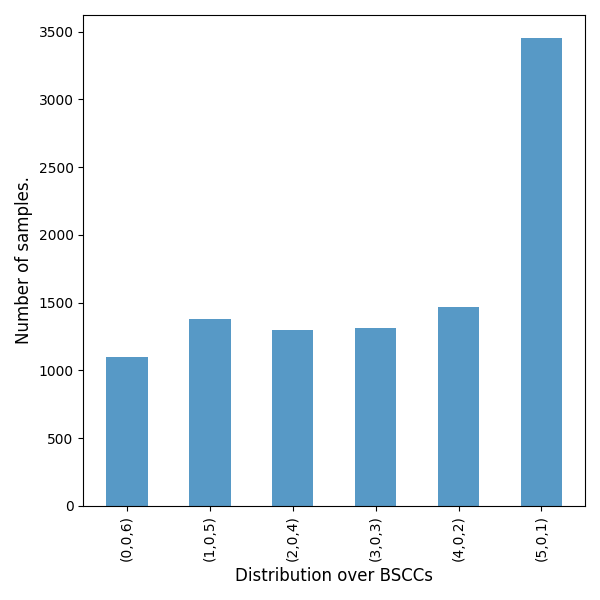
\includegraphics[width=0.45\linewidth]{figures/sir510_data.png}
    \caption{Synthetic data $y_{obs}$ using selected true parameter.}
\end{figure}

\begin{table}[!htb]
    \begin{tabular}{|l|c|l|}
        \hline
        \multicolumn{1}{|c|}{\textbf{SIR(5,1,0)}} & \multicolumn{1}{l|}{\begin{tabular}[c]{@{}l@{}}Rational function\\ SMC\end{tabular}}            & \begin{tabular}[c]{@{}l@{}}Statistical model checking\\ ABC-SMC\end{tabular} \\ \hline
        True parameter                            & \multicolumn{2}{c|}{(0.01724649, 0.06778604)}                                           \\ \hline
        Number of states                          & \multicolumn{2}{c|}{27}                                                                 \\ \hline
        Number of BSCCs                           & \multicolumn{2}{c|}{6}                                                                  \\ \hline
        Target property                           & \multicolumn{2}{c|}{$P_{\geq 0.25} [!(i>2) U^{<6} (i=0)]$}                              \\ \hline
        Synthetic data                            & \multicolumn{2}{c|}{(421,  834, 1126, 1362, 1851, 4406)}                                \\ \hline
        Inferred parameter point                  & \multicolumn{1}{l|}{(0.02307652, 0.06481155)}              & (0.01758384, 0.06535699)   \\ \hline
        L2 distance to true parameter             & \multicolumn{1}{l|}{0.006544985909916083}                  & 0.005519695496673707       \\ \hline
        Run time (hh:mm:ss)                       & \multicolumn{1}{l|}{1:07:36.442146}                        & 3:05:22.61795              \\ \hline
    \end{tabular}
    \caption{SIR(5,1,0) parameter estimation results.}
\end{table}

\begin{figure}[!htb]
    \centering
    \begin{subfigure}{0.48\textwidth}
        \centering
        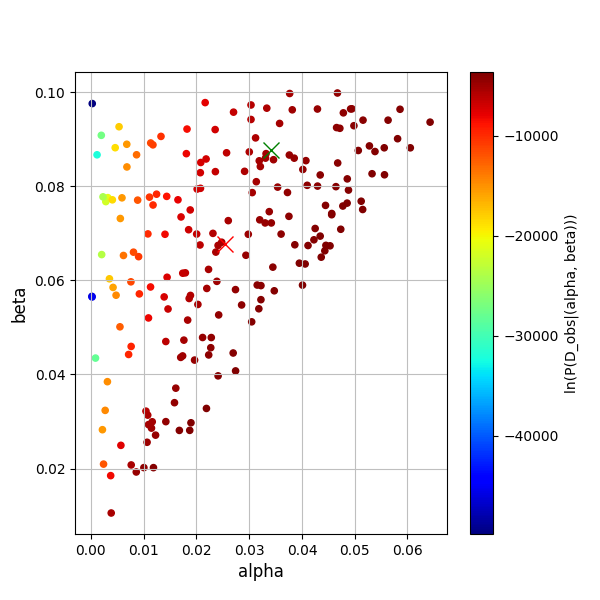
\includegraphics[width=\linewidth]{figures/sir510_rfsmc.png}
        \caption{Sampled particles using Rational Functions SMC}
    \end{subfigure}
    \hfill
    \begin{subfigure}{0.48\textwidth}
        \centering
        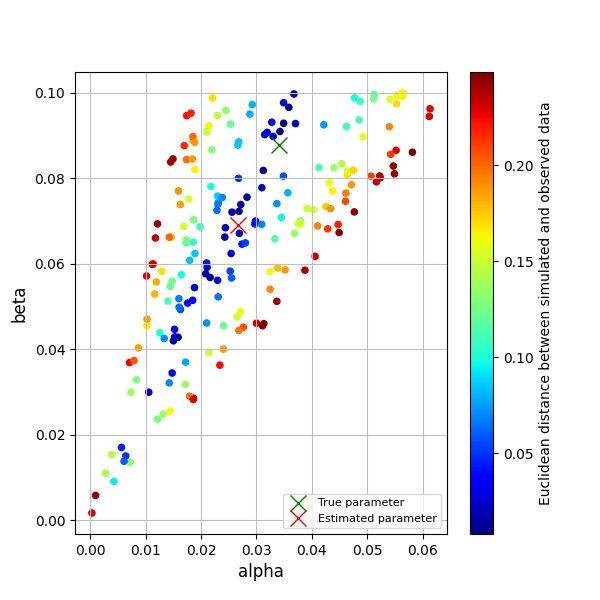
\includegraphics[width=\linewidth]{figures/sir510_abcsmc.png}
        \caption{Sampled particles using Statiscal Model Checking ABC-SMC}
    \end{subfigure}
\end{figure}


\begin{table}[!htb]
    \begin{tabular}{|l|c|l|}
        \hline
        \multicolumn{1}{|c|}{\textbf{SIR(10,1,0)}} & \multicolumn{1}{l|}{\begin{tabular}[c]{@{}l@{}}Rational function\\ SMC\end{tabular}}            & \begin{tabular}[c]{@{}l@{}}Statistical model checking\\ ABC-SMC\end{tabular} \\ \hline
        True parameter                             & \multicolumn{2}{c|}{(0.01724649, 0.06778604)}                                           \\ \hline
        Number of states                           & \multicolumn{2}{c|}{27}                                                                 \\ \hline
        Number of BSCCs                            & \multicolumn{2}{c|}{6}                                                                  \\ \hline
        Target property                            & \multicolumn{2}{c|}{$P_{\geq 0.25} [!(i>2) U^{<6} (i=0)]$}                              \\ \hline
        Synthetic data                             & \multicolumn{2}{c|}{(421,  834, 1126, 1362, 1851, 4406)}                                \\ \hline
        Inferred parameter point                   & \multicolumn{1}{l|}{(0.02307652, 0.06481155)}              & (0.01758384, 0.06535699)   \\ \hline
        L2 distance to true parameter              & \multicolumn{1}{l|}{0.006544985909916083}                  & 0.005519695496673707       \\ \hline
        Run time (hh:mm:ss)                        & \multicolumn{1}{l|}{1:07:36.442146}                        & 3:05:22.61795              \\ \hline
    \end{tabular}
    \caption{SIR(5,1,0) parameter estimation results.}
\end{table}

\begin{figure}[!htb]
    \centering
    \begin{subfigure}{0.48\textwidth}
        \centering
        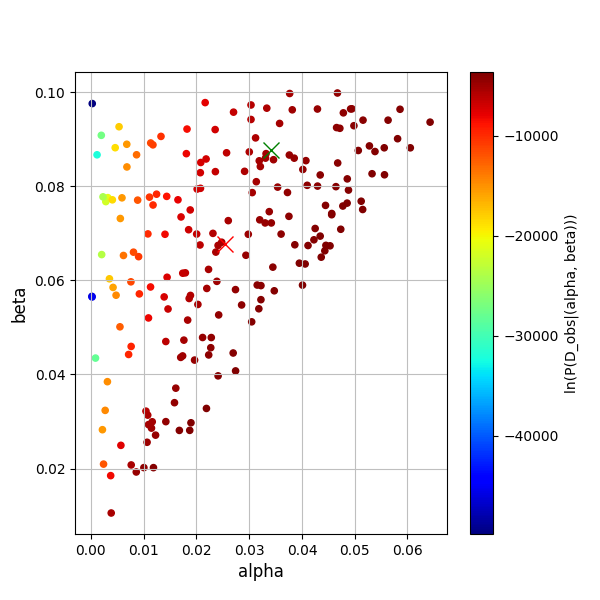
\includegraphics[width=\linewidth]{figures/sir510_rfsmc.png}
        \caption{Sampled particles using Rational Functions SMC}
    \end{subfigure}
    \hfill
    \begin{subfigure}{0.48\textwidth}
        \centering
        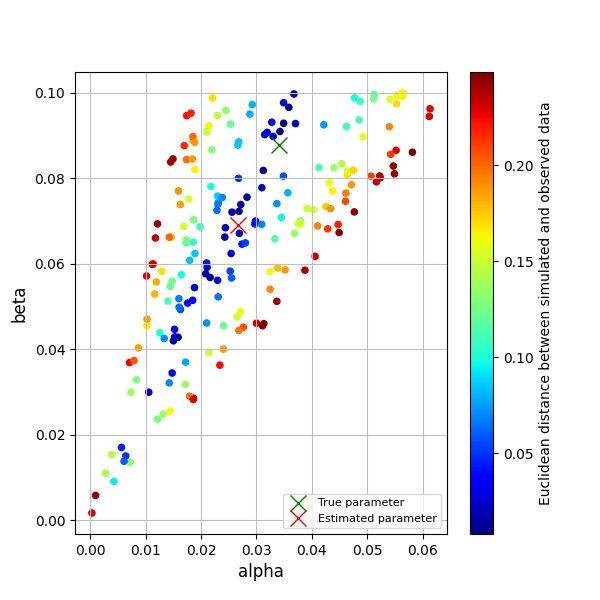
\includegraphics[width=\linewidth]{figures/sir510_abcsmc.png}
        \caption{Sampled particles using Statiscal Model Checking ABC-SMC}
    \end{subfigure}
\end{figure}

\begin{table}[!htb]
    \begin{tabular}{|l|c|l|}
        \hline
        \multicolumn{1}{|c|}{\textbf{SIR(15,1,0)}} & \multicolumn{1}{l|}{\begin{tabular}[c]{@{}l@{}}Rational function\\ SMC\end{tabular}}            & \begin{tabular}[c]{@{}l@{}}Statistical model checking\\ ABC-SMC\end{tabular} \\ \hline
        True parameter                             & \multicolumn{2}{c|}{(0.01724649, 0.06778604)}                                           \\ \hline
        Number of states                           & \multicolumn{2}{c|}{27}                                                                 \\ \hline
        Number of BSCCs                            & \multicolumn{2}{c|}{6}                                                                  \\ \hline
        Target property                            & \multicolumn{2}{c|}{$P_{\geq 0.25} [!(i>2) U^{<6} (i=0)]$}                              \\ \hline
        Synthetic data                             & \multicolumn{2}{c|}{(421,  834, 1126, 1362, 1851, 4406)}                                \\ \hline
        Inferred parameter point                   & \multicolumn{1}{l|}{(0.02307652, 0.06481155)}              & (0.01758384, 0.06535699)   \\ \hline
        L2 distance to true parameter              & \multicolumn{1}{l|}{0.006544985909916083}                  & 0.005519695496673707       \\ \hline
        Run time (hh:mm:ss)                        & \multicolumn{1}{l|}{1:07:36.442146}                        & 3:05:22.61795              \\ \hline
    \end{tabular}
    \caption{SIR(5,1,0) parameter estimation results.}
\end{table}

\begin{figure}[!htb]
    \centering
    \begin{subfigure}{0.48\textwidth}
        \centering
        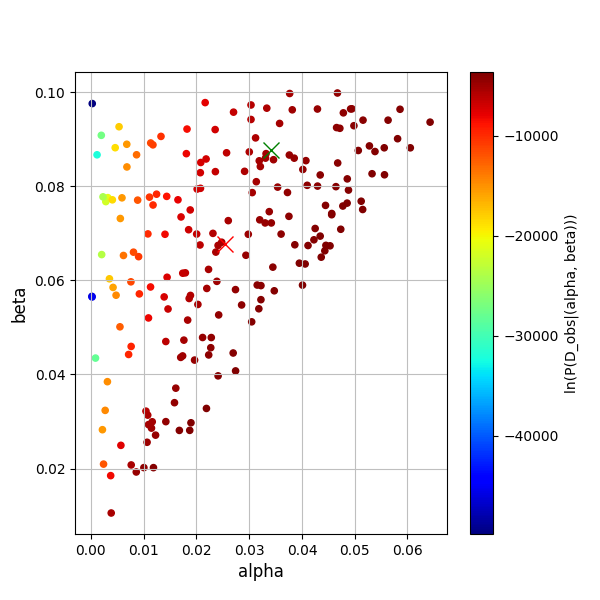
\includegraphics[width=\linewidth]{figures/sir510_rfsmc.png}
        \caption{Sampled particles using Rational Functions SMC}
    \end{subfigure}
    \hfill
    \begin{subfigure}{0.48\textwidth}
        \centering
        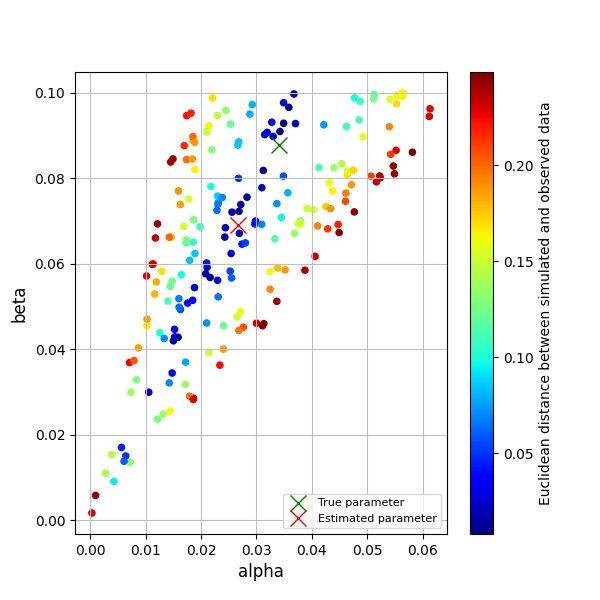
\includegraphics[width=\linewidth]{figures/sir510_abcsmc.png}
        \caption{Sampled particles using Statiscal Model Checking ABC-SMC}
    \end{subfigure}
\end{figure}

\begin{table}[!htb]
    \begin{tabular}{|l|c|l|}
        \hline
        \multicolumn{1}{|c|}{\textbf{SIR(10,1,0)}, BSCC merged} & \multicolumn{1}{l|}{\begin{tabular}[c]{@{}l@{}}Rational function\\ SMC\end{tabular}}            & \begin{tabular}[c]{@{}l@{}}Statistical model checking\\ ABC-SMC\end{tabular} \\ \hline
        True parameter                                          & \multicolumn{2}{c|}{(0.01724649, 0.06778604)}                                           \\ \hline
        Number of states                                        & \multicolumn{2}{c|}{27}                                                                 \\ \hline
        Number of BSCCs                                         & \multicolumn{2}{c|}{6}                                                                  \\ \hline
        Target property                                         & \multicolumn{2}{c|}{$P_{\geq 0.25} [!(i>2) U^{<6} (i=0)]$}                              \\ \hline
        Synthetic data                                          & \multicolumn{2}{c|}{(421,  834, 1126, 1362, 1851, 4406)}                                \\ \hline
        Inferred parameter point                                & \multicolumn{1}{l|}{(0.02307652, 0.06481155)}              & (0.01758384, 0.06535699)   \\ \hline
        L2 distance to true parameter                           & \multicolumn{1}{l|}{0.006544985909916083}                  & 0.005519695496673707       \\ \hline
        Run time (hh:mm:ss)                                     & \multicolumn{1}{l|}{1:07:36.442146}                        & 3:05:22.61795              \\ \hline
    \end{tabular}
    \caption{SIR(5,1,0) parameter estimation results.}
\end{table}

\begin{figure}[!htb]
    \centering
    \begin{subfigure}{0.48\textwidth}
        \centering
        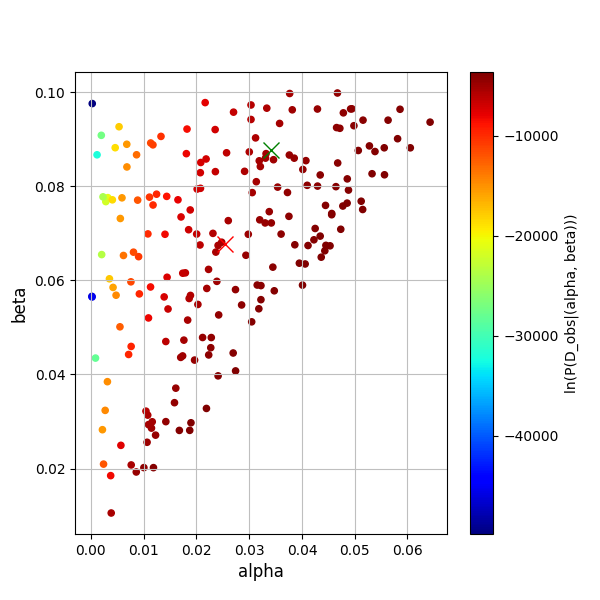
\includegraphics[width=\linewidth]{figures/sir510_rfsmc.png}
        \caption{Sampled particles using Rational Functions SMC}
    \end{subfigure}
    \hfill
    \begin{subfigure}{0.48\textwidth}
        \centering
        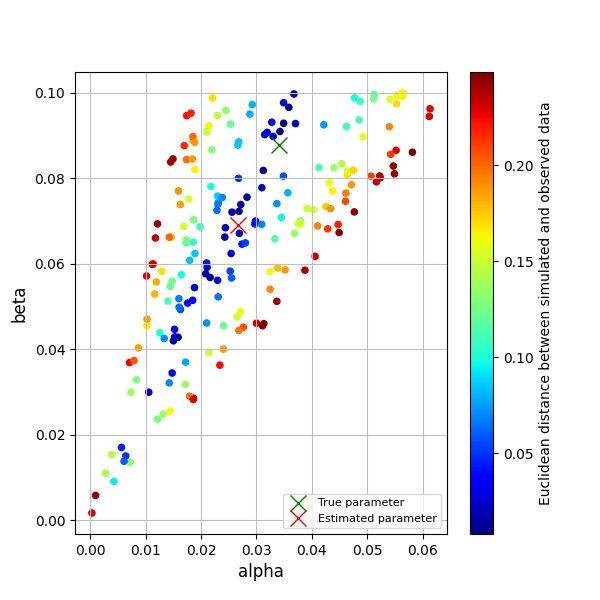
\includegraphics[width=\linewidth]{figures/sir510_abcsmc.png}
        \caption{Sampled particles using Statiscal Model Checking ABC-SMC}
    \end{subfigure}
\end{figure}

\begin{table}[!htb]
    \begin{tabular}{|l|c|l|}
        \hline
        \multicolumn{1}{|c|}{\textbf{SIR(10,1,0)}, BSCC merged} & \multicolumn{1}{l|}{\begin{tabular}[c]{@{}l@{}}Rational function\\ SMC\end{tabular}}            & \begin{tabular}[c]{@{}l@{}}Statistical model checking\\ ABC-SMC\end{tabular} \\ \hline
        True parameter                                          & \multicolumn{2}{c|}{(0.01724649, 0.06778604)}                                           \\ \hline
        Number of states                                        & \multicolumn{2}{c|}{27}                                                                 \\ \hline
        Number of BSCCs                                         & \multicolumn{2}{c|}{6}                                                                  \\ \hline
        Target property                                         & \multicolumn{2}{c|}{$P_{\geq 0.25} [!(i>2) U^{<6} (i=0)]$}                              \\ \hline
        Synthetic data                                          & \multicolumn{2}{c|}{(421,  834, 1126, 1362, 1851, 4406)}                                \\ \hline
        Inferred parameter point                                & \multicolumn{1}{l|}{(0.02307652, 0.06481155)}              & (0.01758384, 0.06535699)   \\ \hline
        L2 distance to true parameter                           & \multicolumn{1}{l|}{0.006544985909916083}                  & 0.005519695496673707       \\ \hline
        Run time (hh:mm:ss)                                     & \multicolumn{1}{l|}{1:07:36.442146}                        & 3:05:22.61795              \\ \hline
    \end{tabular}
    \caption{SIR(5,1,0) parameter estimation results.}
\end{table}

\begin{figure}[!htb]
    \centering
    \begin{subfigure}{0.48\textwidth}
        \centering
        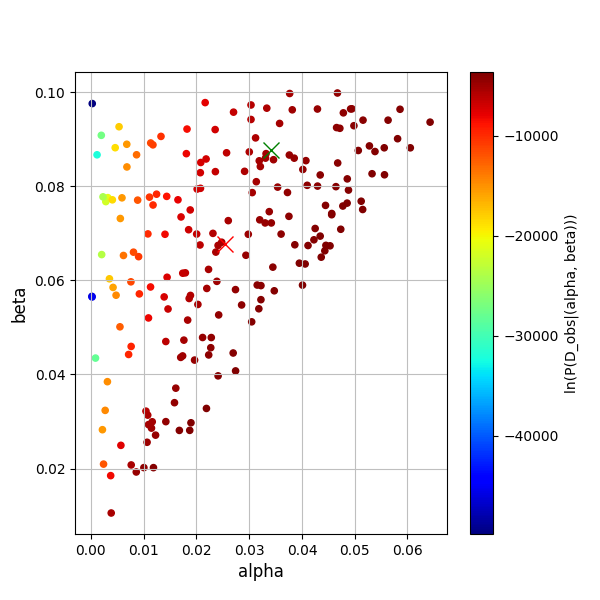
\includegraphics[width=\linewidth]{figures/sir510_rfsmc.png}
        \caption{Sampled particles using Rational Functions SMC}
    \end{subfigure}
    \hfill
    \begin{subfigure}{0.48\textwidth}
        \centering
        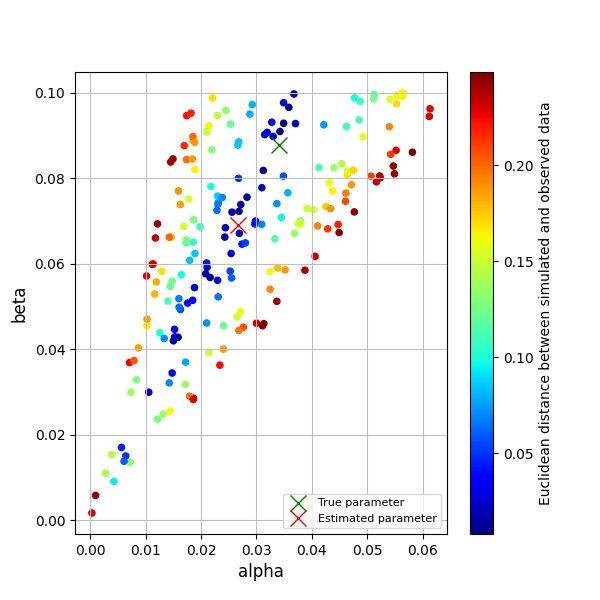
\includegraphics[width=\linewidth]{figures/sir510_abcsmc.png}
        \caption{Sampled particles using Statiscal Model Checking ABC-SMC}
    \end{subfigure}
\end{figure}

\subsubsection{Parameter synthesis with uncertainty}

\subsection{Discussion}
This experiment shows good results.
